\subsubsection{Crossover}
\label{sec:bg:gp:var:cx}
  Variation operators in Genetic Programming (GP) must maintain the syntactic 
  correctness of the programs or individuals.
  For crossover, this implies that the resultant offspring must be syntactically
  correct programs.

  The crossover operator used in Genetic Algorithms (GAs), described in 
  \vref{sec:bg:ga:var:cx}, is not typically suitable for GP, as it does not 
  guarantee the syntactic correctness of the resulting individuals.
  Though there could be instances where the crossover operator used in GAs is
  applicable to GP, as depicted in \vref{chap:beacon}, these are not common
  scenarios.

  The choice of operator in GP depends on the representation of the individuals.

  For tree-based GP, the fundamental crossover operator is the \emph{subtree 
  crossover}, referenced in \vref{sec:keen:operators:crossover:single_node}.

  This operator selects a random node from each parent and exchanges the 
  subtrees rooted at these nodes.
  Usually, a constraint similar to the one used for generating the initial
  population is applied to this operator to prevent the creation of overly large
  trees.

  Assuming we select two individuals, \(\mathbf{I}_1\) and \(\mathbf{I}_2\), 
  from the population, the subtree crossover operator chooses a random node from 
  each individual, say \(\clubsuit = 7\) from \(\mathbf{I}_1\) and 
  \(\diamondsuit = x^2\) from \(\mathbf{I}_2\).
  The subtrees rooted at these nodes are then interchanged, as shown below:

  \begin{table}[H]
    \centering
    \begin{tabular}{rrl}                    
        & \(\chi(\mathbf{I}_2,\,\mathbf{I}_4)\)
        & \(= \chi(\clubsuit - (5 + \sin(x)),\,5\diamondsuit)\)
      \\
        &   
        & \(= (\diamondsuit - (5 + \sin(x)),\,5\clubsuit)\)
      \\
      \(\Leftrightarrow\)
        & \((\mathbf{O}_1,\,\mathbf{O}_2)\)
        & \(= (x^2 - (5 + \sin(x)),\,5 \cdot 7)\)
    \end{tabular}
  \end{table}

  where \(\chi\) signifies the subtree crossover operator between two 
  individuals.
  The crossover of \(\mathbf{I}_1\) and \(\mathbf{I}_2\) is depicted in
  \vref{fig:bg:gp:variation:crossover:subtree}.

  \begin{figure}[ht!]
    \centering
    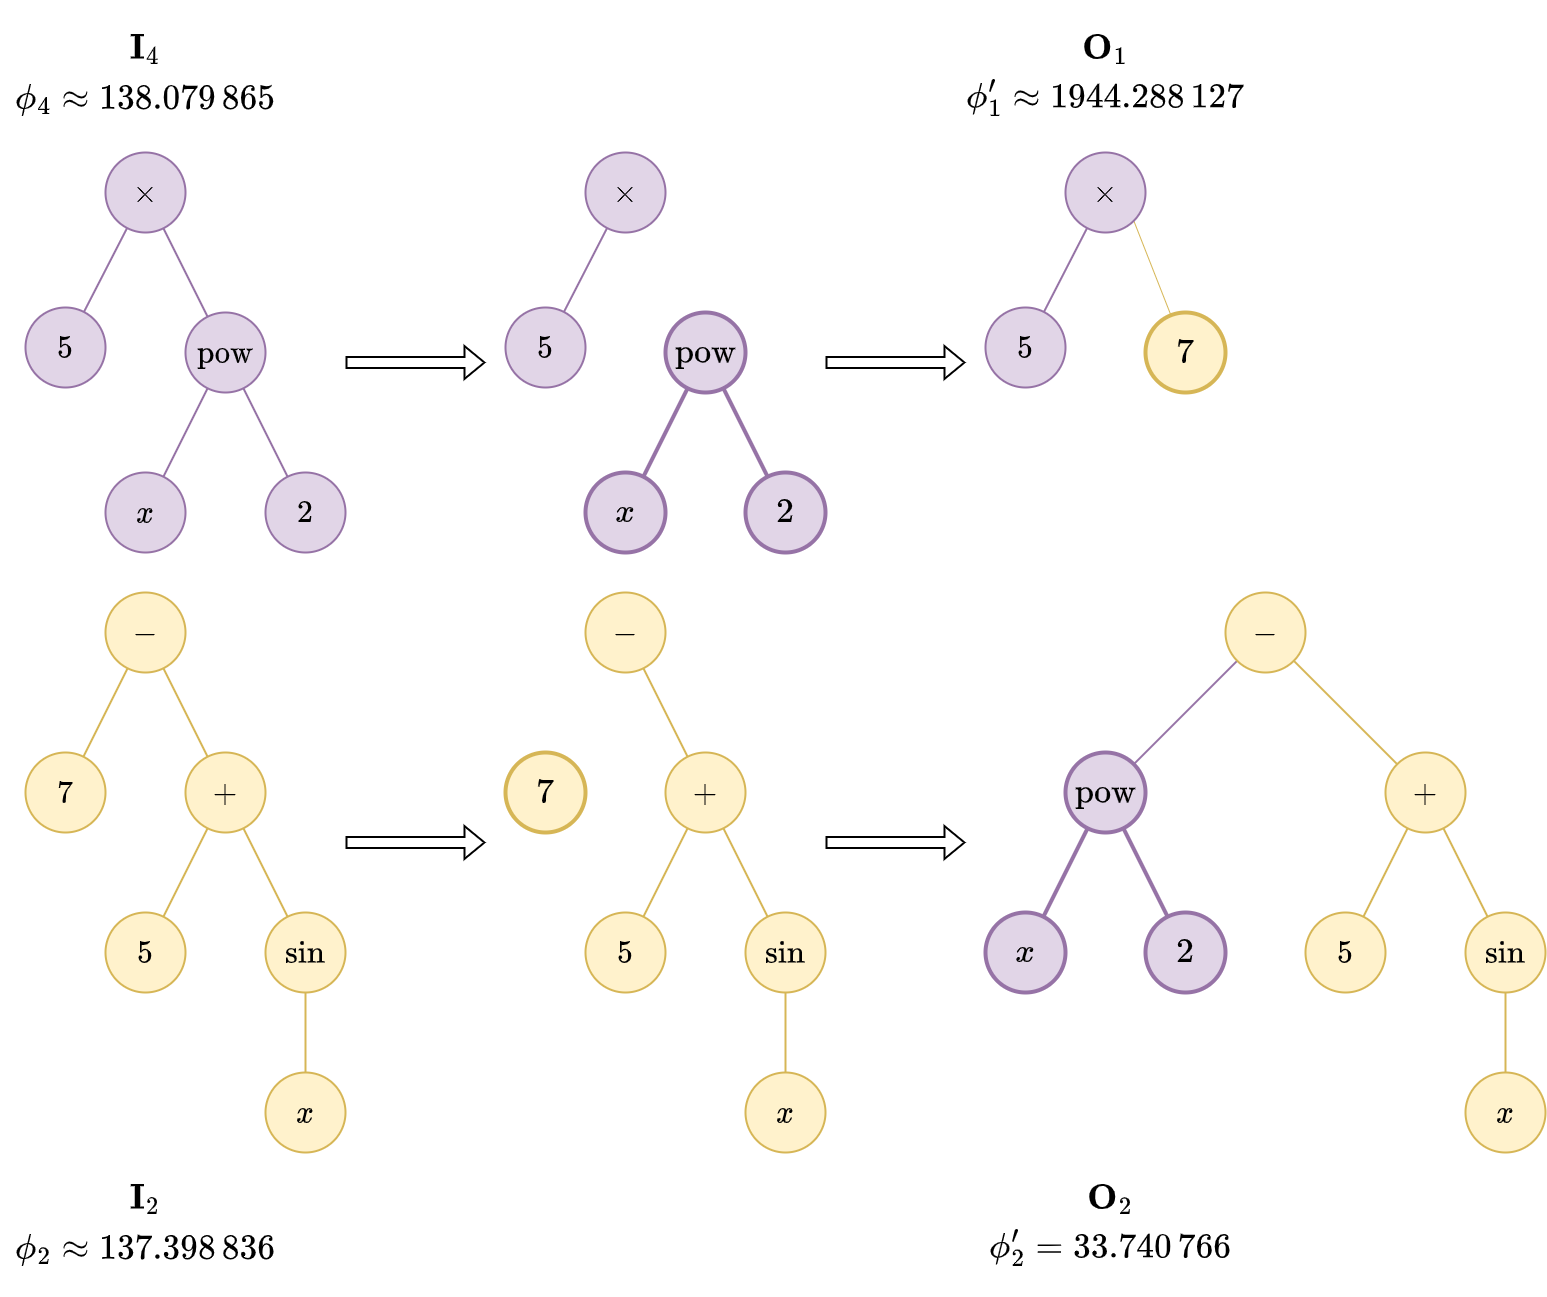
\includegraphics[width=0.8\textwidth]
      {img/theoretical_framework/GP Crossover.png}
    \caption{
      Crossing over of \(\mathbf{I}_2 = 7 - (5 + \sin(x))\) and 
      \(\mathbf{I}_4 = 5x^2\), producing \(\mathbf{O}_1 = x^2 - (5 + \sin(x))\) 
      and \(\mathbf{O}_2 = 5 \cdot 7\).
    }
    \label{fig:bg:gp:variation:crossover:subtree}
  \end{figure}


    Following the application of the subtree crossover operator, the fitness of 
    the individuals in the population is evaluated as shown in 
    \vref{tab:bg:gp:variation:crossover:subtree:fitness}.
    A summary of the population's fitness is given in 
    \vref{tab:bg:gp:variation:crossover:subtree:fitness:summary}.

    \subimport{./}{tab-bg-gp-variation-crossover-subtree-fitness.tex}
    \subimport{./}{tab-bg-gp-variation-crossover-subtree-fitness-summary.tex}

    A notable improvement in the population's fitness is observed after the 
    application of the subtree crossover operator.
    Comparing the results from 
    \vref{tab:bg:gp:sym:init:pop:summary}, we find that the 
    average fitness (or error) has dropped from \(44\,551.063\,525\) to 
    \(611.837\,999\), equating to an improvement of approximately \(98.627\%\).

  \[
    \frac{\bar{\Phi}_i - \bar{\Phi}_X}{\bar{\Phi}_i}
     = \frac{44\,551.063\,525 - 611.837\,999}{44\,551.063\,525} \approx 98.627\%
  \]

  where \(\bar{\Phi}_i\) is the average fitness of the population after
  initialization and \(\bar{\Phi}_X\) is the average fitness of the population
  after applying the subtree crossover operator.

  A reduction in the population's fitness standard deviation, from 
  \(76\,814.062\,197\) to \(776.701\,997\), is also seen.
  This decrease of around \(98.989\%\) indicates that the population's diversity
  has reduced.

  \[
    \frac{\sigma_i - \sigma_X}{\sigma_i}
     = \frac{76\,814.062\,197 - 776.701\,997}{76\,814.062\,197} \approx 98.989\%
  \]

  where \(\sigma_i\) is the standard deviation of the fitness of the population
  after initialization and \(\sigma_X\) is the standard deviation of the
  fitness of the population after applying the subtree crossover operator.
  
  Diversity here is a measure of population's dispersion, and a decline in 
  diversity may signal that the population is not converging towards a solution 
  (too much diversity) or is converging prematurely (too little diversity).


  In the following section, we discuss the mutation operator, which can be used 
  to introduce diversity into the population, thereby preventing premature 
  convergence.
